\documentclass{standalone}
\usepackage{tikz}
\usetikzlibrary{patterns, positioning}
\usepackage[sfdefault]{ClearSans} %% option 'sfdefault' activates Clear Sans as the default text font
\usepackage[T1]{fontenc}

\begin{document}
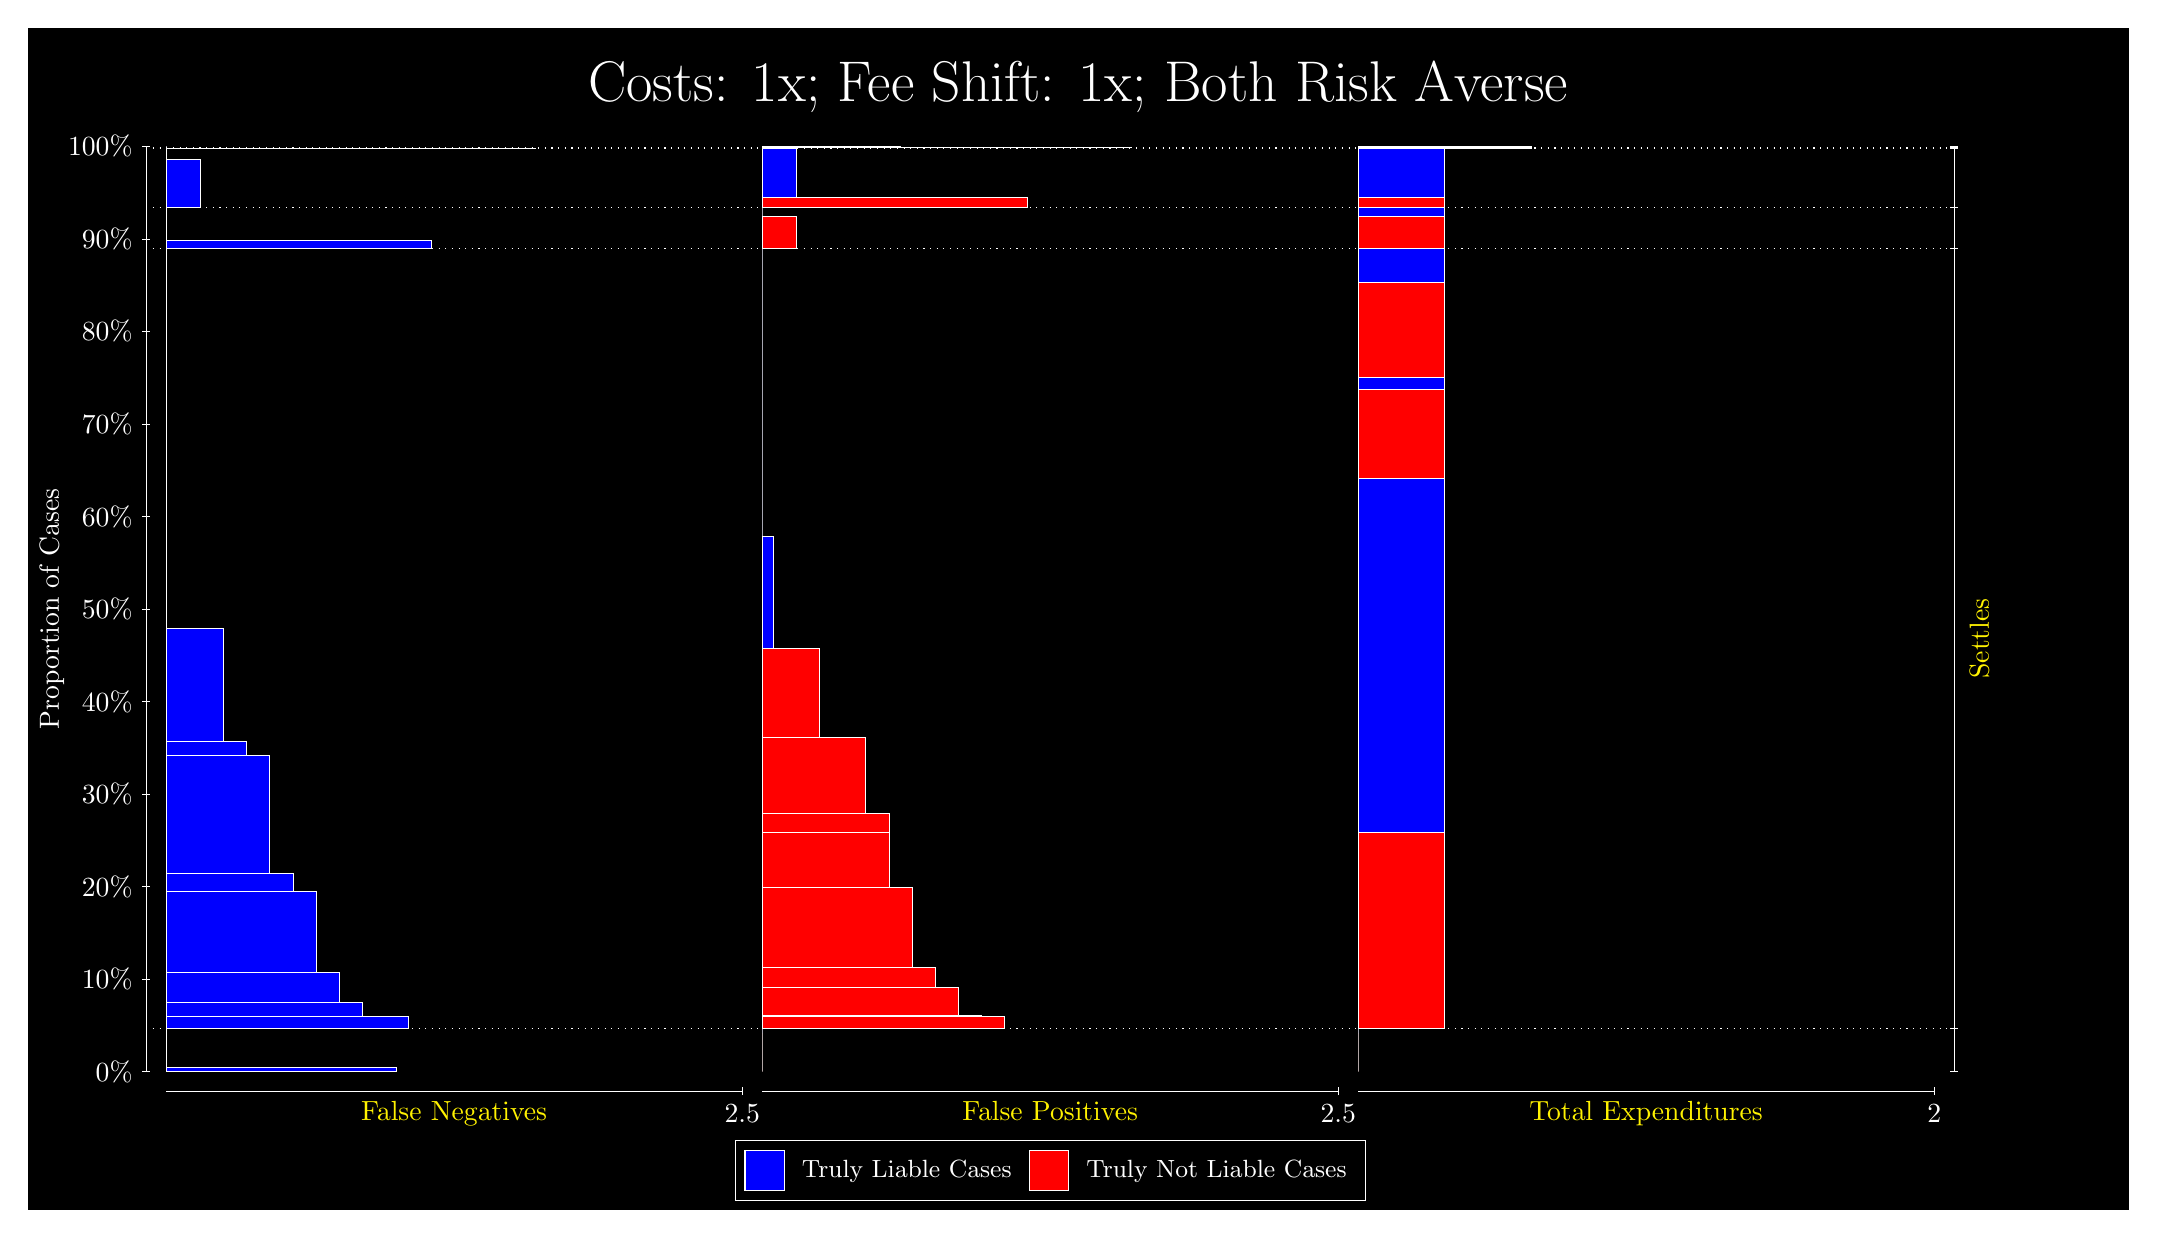
\begin{tikzpicture}
\draw[fill=black] (0,0) rectangle (26.667,15);
\draw[text=white] (0,13.5) rectangle (26.667,15) node[midway] {\huge Costs: 1x; Fee Shift: 1x; Both Risk Averse};
\draw[white, very thin] (1.5,1.75) -- (1.5,13.5);
\node[rotate=90, text=white, anchor=center] at (0.3, 7.625) {Proportion of Cases};
\draw[white, very thin] (1.45,1.75) -- (1.55,1.75);
\node[text=white, anchor=east] at (1.45, 1.75) {0\%};
\draw[white, very thin] (1.45,2.925) -- (1.55,2.925);
\node[text=white, anchor=east] at (1.45, 2.925) {10\%};
\draw[white, very thin] (1.45,4.1) -- (1.55,4.1);
\node[text=white, anchor=east] at (1.45, 4.1) {20\%};
\draw[white, very thin] (1.45,5.275) -- (1.55,5.275);
\node[text=white, anchor=east] at (1.45, 5.275) {30\%};
\draw[white, very thin] (1.45,6.45) -- (1.55,6.45);
\node[text=white, anchor=east] at (1.45, 6.45) {40\%};
\draw[white, very thin] (1.45,7.625) -- (1.55,7.625);
\node[text=white, anchor=east] at (1.45, 7.625) {50\%};
\draw[white, very thin] (1.45,8.8) -- (1.55,8.8);
\node[text=white, anchor=east] at (1.45, 8.8) {60\%};
\draw[white, very thin] (1.45,9.975) -- (1.55,9.975);
\node[text=white, anchor=east] at (1.45, 9.975) {70\%};
\draw[white, very thin] (1.45,11.15) -- (1.55,11.15);
\node[text=white, anchor=east] at (1.45, 11.15) {80\%};
\draw[white, very thin] (1.45,12.325) -- (1.55,12.325);
\node[text=white, anchor=east] at (1.45, 12.325) {90\%};
\draw[white, very thin] (1.45,13.5) -- (1.55,13.5);
\node[text=white, anchor=east] at (1.45, 13.5) {100\%};

\draw[white, very thin] (24.457,1.75) -- (24.457,13.5);
\draw[white, very thin] (24.407,1.75) -- (24.507,1.75);
\node[anchor=west] at (24.407, 1.75) {};
\draw[white, very thin] (24.407,2.2966) -- (24.507,2.2966);
\node[anchor=west] at (24.407, 2.2966) {};
\draw[white, very thin] (24.407,12.2) -- (24.507,12.2);
\node[anchor=west] at (24.407, 12.2) {};
\draw[white, very thin] (24.407,12.724) -- (24.507,12.724);
\node[anchor=west] at (24.407, 12.724) {};
\draw[white, very thin] (24.407,13.473) -- (24.507,13.473);
\node[anchor=west] at (24.407, 13.473) {};
\draw[white, very thin] (24.407,13.486) -- (24.507,13.486);
\node[anchor=west] at (24.407, 13.486) {};
\draw[white, very thin] (24.407,13.5) -- (24.507,13.5);
\node[anchor=west] at (24.407, 13.5) {};

\draw[white, very thin, fill=blue] (1.75,1.75) rectangle (4.6775,1.8075);
\draw[white, very thin, fill=red] (1.75,1.8075) rectangle (1.75,2.2966);
\draw[white, very thin, fill=blue] (1.75,2.2966) rectangle (4.8239,2.4532);
\draw[white, very thin, fill=blue] (1.75,2.4532) rectangle (4.2384,2.6234);
\draw[white, very thin, fill=blue] (1.75,2.6234) rectangle (3.9457,3.0086);
\draw[white, very thin, fill=blue] (1.75,3.0086) rectangle (3.6529,4.0352);
\draw[white, very thin, fill=blue] (1.75,4.0352) rectangle (3.3602,4.2615);
\draw[white, very thin, fill=blue] (1.75,4.2615) rectangle (3.0674,5.7712);
\draw[white, very thin, fill=blue] (1.75,5.7712) rectangle (2.7746,5.9423);
\draw[white, very thin, fill=blue] (1.75,5.9423) rectangle (2.4819,7.3757);
\draw[white, very thin, fill=red] (1.75,7.3757) rectangle (1.75,12.2);
\draw[white, very thin, fill=blue] (1.75,12.2) rectangle (5.1167,12.308);
\draw[white, very thin, fill=red] (1.75,12.308) rectangle (1.75,12.724);
\draw[white, very thin, fill=blue] (1.75,12.724) rectangle (2.1891,13.34);
\draw[white, very thin, fill=red] (1.75,13.34) rectangle (1.75,13.473);
\draw[white, very thin, fill=blue] (1.75,13.473) rectangle (6.4341,13.478);
\draw[white, very thin, fill=red] (1.75,13.478) rectangle (1.75,13.486);
\draw[white, very thin, fill=red] (1.75,13.486) rectangle (1.75,13.491);
\draw[white, very thin, fill=blue] (1.75,13.491) rectangle (1.75,13.5);
\draw[white, very thin, fill=red] (9.3189,1.75) rectangle (9.3189,2.2391);
\draw[white, very thin, fill=blue] (9.3189,2.2391) rectangle (9.3189,2.2966);
\draw[white, very thin, fill=red] (9.3189,2.2966) rectangle (12.393,2.4522);
\draw[white, very thin, fill=red] (9.3189,2.4522) rectangle (12.1,2.4688);
\draw[white, very thin, fill=red] (9.3189,2.4688) rectangle (11.807,2.8197);
\draw[white, very thin, fill=red] (9.3189,2.8197) rectangle (11.515,3.0692);
\draw[white, very thin, fill=red] (9.3189,3.0692) rectangle (11.222,4.0933);
\draw[white, very thin, fill=red] (9.3189,4.0933) rectangle (10.929,4.7908);
\draw[white, very thin, fill=red] (9.3189,4.7908) rectangle (10.929,5.0345);
\draw[white, very thin, fill=red] (9.3189,5.0345) rectangle (10.636,5.9939);
\draw[white, very thin, fill=red] (9.3189,5.9939) rectangle (10.051,7.1205);
\draw[white, very thin, fill=blue] (9.3189,7.1205) rectangle (9.4652,8.5539);
\draw[white, very thin, fill=blue] (9.3189,8.5539) rectangle (9.3189,12.2);
\draw[white, very thin, fill=red] (9.3189,12.2) rectangle (9.758,12.615);
\draw[white, very thin, fill=blue] (9.3189,12.615) rectangle (9.3189,12.724);
\draw[white, very thin, fill=red] (9.3189,12.724) rectangle (12.686,12.857);
\draw[white, very thin, fill=blue] (9.3189,12.857) rectangle (9.758,13.473);
\draw[white, very thin, fill=red] (9.3189,13.473) rectangle (9.3189,13.482);
\draw[white, very thin, fill=blue] (9.3189,13.482) rectangle (9.3189,13.486);
\draw[white, very thin, fill=red] (9.3189,13.486) rectangle (14.003,13.491);
\draw[white, very thin, fill=blue] (9.3189,13.491) rectangle (11.075,13.5);
\draw[white, very thin, fill=red] (16.888,1.75) rectangle (16.888,2.2391);
\draw[white, very thin, fill=blue] (16.888,2.2391) rectangle (16.888,2.2966);
\draw[white, very thin, fill=red] (16.888,2.2966) rectangle (17.986,4.7908);
\draw[white, very thin, fill=blue] (16.888,4.7908) rectangle (17.986,9.283);
\draw[white, very thin, fill=red] (16.888,9.283) rectangle (17.986,10.41);
\draw[white, very thin, fill=blue] (16.888,10.41) rectangle (17.986,10.566);
\draw[white, very thin, fill=red] (16.888,10.566) rectangle (17.986,11.769);
\draw[white, very thin, fill=blue] (16.888,11.769) rectangle (17.986,12.2);
\draw[white, very thin, fill=red] (16.888,12.2) rectangle (17.986,12.615);
\draw[white, very thin, fill=blue] (16.888,12.615) rectangle (17.986,12.724);
\draw[white, very thin, fill=red] (16.888,12.724) rectangle (17.986,12.857);
\draw[white, very thin, fill=blue] (16.888,12.857) rectangle (17.986,13.473);
\draw[white, very thin, fill=red] (16.888,13.473) rectangle (19.083,13.482);
\draw[white, very thin, fill=blue] (16.888,13.482) rectangle (19.083,13.486);
\draw[white, very thin, fill=red] (16.888,13.486) rectangle (19.083,13.491);
\draw[white, very thin, fill=blue] (16.888,13.491) rectangle (19.083,13.5);
\draw[white, dotted] (1.5,2.2966) -- (24.457,2.2966);
\draw[white, dotted] (1.5,12.2) -- (24.457,12.2);
\draw[white, dotted] (1.5,12.724) -- (24.457,12.724);
\draw[white, dotted] (1.5,13.473) -- (24.457,13.473);
\draw[white, dotted] (1.5,13.486) -- (24.457,13.486);
\draw[white, very thin] (1.75,1.5) -- (9.0689,1.5);
\node[text=yellow, anchor=north] at (5.4094, 1.5) {False Negatives};
\draw[white, very thin] (9.0689,1.45) -- (9.0689,1.55);
\node[text=white, anchor=north] at (9.0689, 1.45) {2.5};

\draw[white, very thin] (9.3189,1.5) -- (16.638,1.5);
\node[text=yellow, anchor=north] at (12.978, 1.5) {False Positives};
\draw[white, very thin] (16.638,1.45) -- (16.638,1.55);
\node[text=white, anchor=north] at (16.638, 1.45) {2.5};

\draw[white, very thin] (16.888,1.5) -- (24.207,1.5);
\node[text=yellow, anchor=north] at (20.547, 1.5) {Total Expenditures};
\draw[white, very thin] (24.207,1.45) -- (24.207,1.55);
\node[text=white, anchor=north] at (24.207, 1.45) {2};


\node[text=yellow, centered, rotate=90] at (24.777, 7.2481) {Settles};





\draw (12.978300999999998,1.5) node[draw=none] (baseCoordinate) {};
\begin{scope}[align=center]
        \matrix[scale=0.5, draw=white, below=0.5cm of baseCoordinate, nodes={draw}, column sep=0.1cm]{
            \node[rectangle, draw, minimum width=0.5cm, minimum height=0.5cm, fill=blue] {}; &
            \node[draw=none, font=\small, text=white] (B) {Truly Liable Cases}; &
            \node[rectangle, draw, minimum width=0.5cm, minimum height=0.5cm, fill=red] {}; &
            \node[draw=none, font=\small, text=white] (B) {Truly Not Liable Cases}; \\
            };
\end{scope}

\end{tikzpicture}
\end{document}